\documentclass{beamer}

% ************* Preamble *************************** 
% Language setting
% Replace `english' with e.g. `spanish' to change the document language
\usepackage[english]{babel}

% Useful packages
\usepackage{amsmath}
% \usepackage{graphicx} %already loaded by beamer document class
\graphicspath{{../figures/}}
% \usepackage{hyperref} %already loaded by beamer document class
\usepackage{blindtext} % to generate 2 pages of text

% Dont use caption/ subcaption in beamer, use columns instead.
\usepackage[compatibility=false]{caption} % for subfigures (panels)
\usepackage{subcaption} % for subfigures (panels)
% \setbeamertemplate{caption}[numbered] %to get figures to be numbered in beamer class

% Biblatex (options taken from Igors Github, is it equal to JoF style?)
\usepackage[
    backend=biber,
    style=bwl-FU,
    url=false,
    doi=false,
    eprint=false
]{biblatex}
% \addbibresource{references.bib}


% Title
\title{Presentation title}

% \author[test]{Egemen Erdogdu\thanks{Egemen Erdogdu, University of Zurich, Rämistrasse 71, 8006 Zürich} \and Jonas Schmidiger\thanks{Jonas Schmidiger, University of Zurich, Rämistrasse 71, 8006 Zürich} \and Mathias Ruoss\thanks{Mathias Ruoss, University of Zurich, Rämistrasse 71, 8006 Zürich}}
\author[E. Erdogdu, J. Schmidiger, M. Ruoss] % (optional, for multiple authors)
{E. Erdogdu\inst{1} \and J. Schmidiger\inst{2} \and M. Ruoss\inst{3}}

\institute[UZH] % (optional)
{
  \inst{1}%
  Faculty of Banking and Finance\\
  Very Famous University
  \and
  \inst{2}%
  Faculty of Banking and Finance\\
  Very Famous University
  \and
  \inst{3}%
  Faculty of Banking and Finance\\
  Very Famous University
}
\date{\today}


% \usetheme[]{Warsaw}
% \usecolortheme{orchid}

% ***********************************************
\begin{document}

\frame{\titlepage}

% % Table of Contents
% \begin{frame}
%     \frametitle{Table of Contents}
%     \tableofcontents    
% \end{frame}

% \section{Section 1}
\begin{frame}
    \frametitle{A theorem}
    \framesubtitle{Frame subtitle}
    \begin{theorem}
        $a^2 + b^2 = c^2$
    \end{theorem}
\end{frame}

% \section{Section 2}
\begin{frame}
    \frametitle{Some equations}
    \framesubtitle{Frame subtitle}
    % \begin{equation}
        \begin{align}
            y + x = 3\\
            y + 3 + 4 = 10\\
            y + \mathbf{x} + Z = 3
        \end{align}
    % \end{equation}
\end{frame}

% \section{Section 3}
\begin{frame}
    \frametitle{A figure with two panels}
    \framesubtitle{A Subtitle}
    \begin{figure}
    \centering
      \begin{subfigure}{0.45\textwidth}
        \centering
        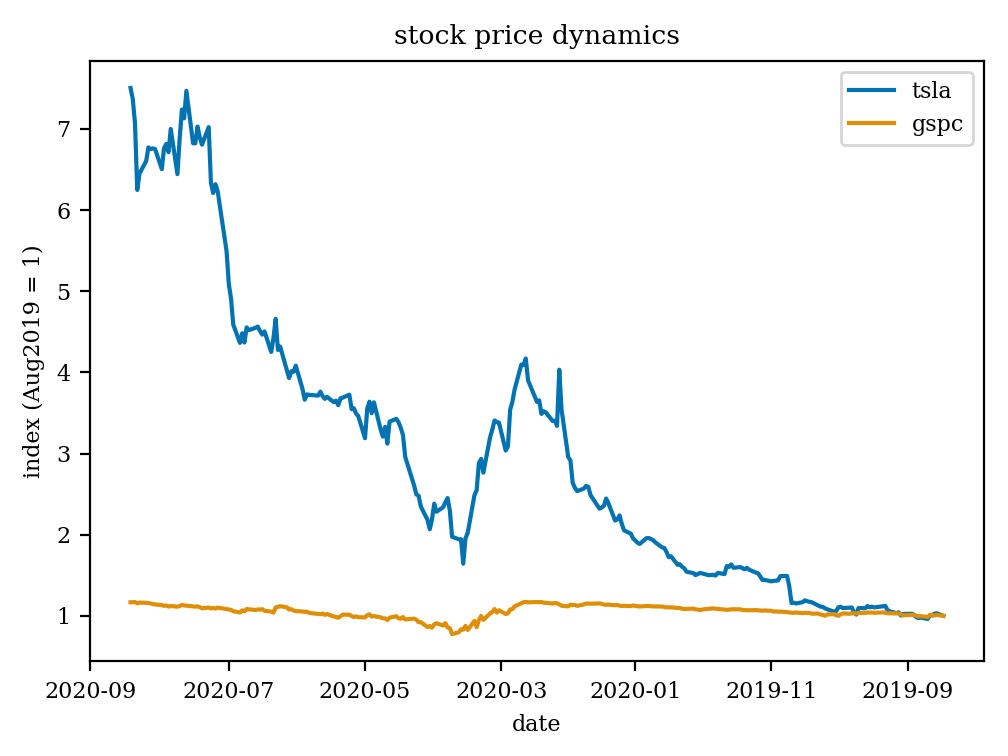
\includegraphics[width=\textwidth]{stock-index-weird-plot}
        \caption{First subfigure}
        \label{fig:a}
      \end{subfigure}\hfill
      \begin{subfigure}{0.45\textwidth}
        \centering
        % Figures taken from igors github
        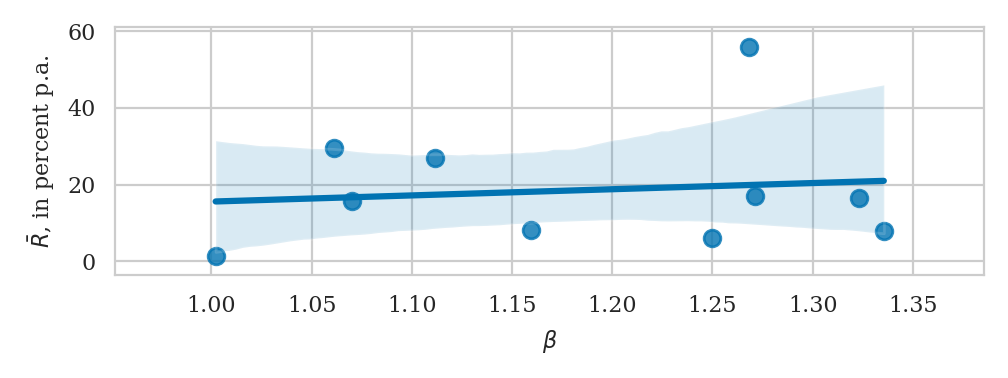
\includegraphics[width=\textwidth]{beta-vs-mu}
        \caption{Second subfigure}
        \label{fig:b}
      \end{subfigure}\\
    \caption{Two panels side by side}\label{fig:stock-beta-comparison}
    \end{figure}
\end{frame}


\begin{frame}
    \frametitle{Another figure with two panels aligned}
    \framesubtitle{Another subtitle}
    \begin{figure}[H]
        \centering
        \subcaptionbox{First subfigure}%
          [.45\linewidth]{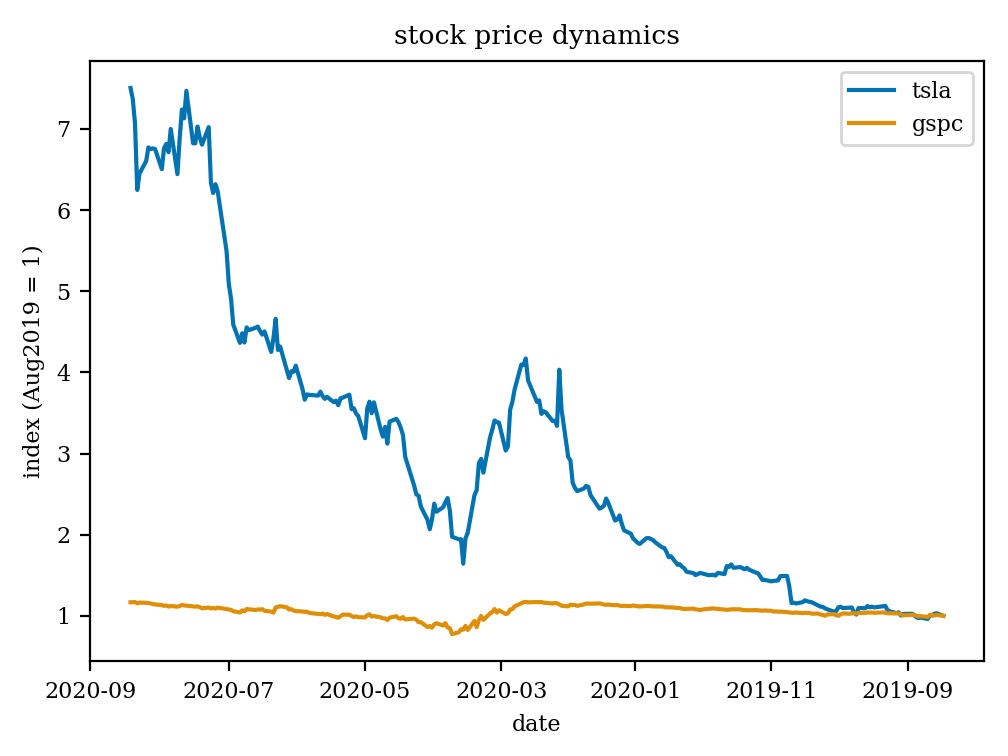
\includegraphics[height=3.5cm]{stock-index-weird-plot.png}}
        \subcaptionbox{Second subfigure}
          [.45\linewidth]{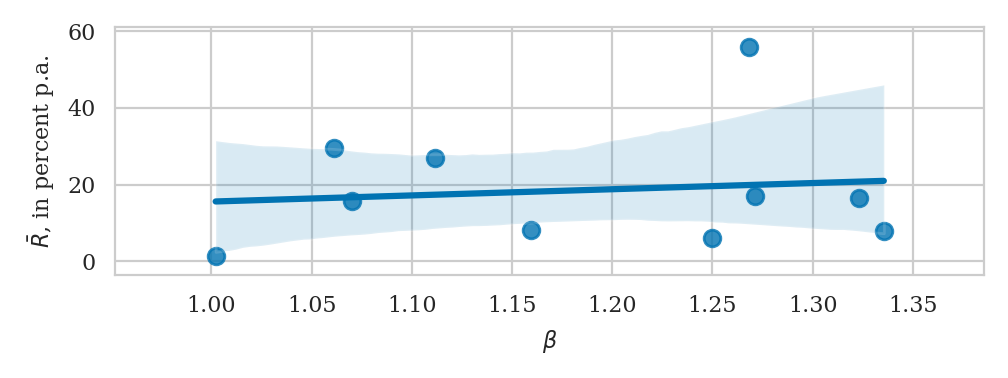
\includegraphics[height=2cm]{beta-vs-mu.png}}
    \caption{Two panels side by side}    
    \end{figure}        
\end{frame}

% \begin{frame}
%     \frametitle{Another figure with two panels}
%     \framesubtitle{Frame subtitle}
%     \begin{figure}
%         % \setbeamerfont{caption}{size=\footnotesize}
%         \begin{columns}[onlytextwidth]
%             \begin{column}{.45\textwidth}
%                 \centering
%                 % Figures taken from igors github
%                 \begin{figure}
%                     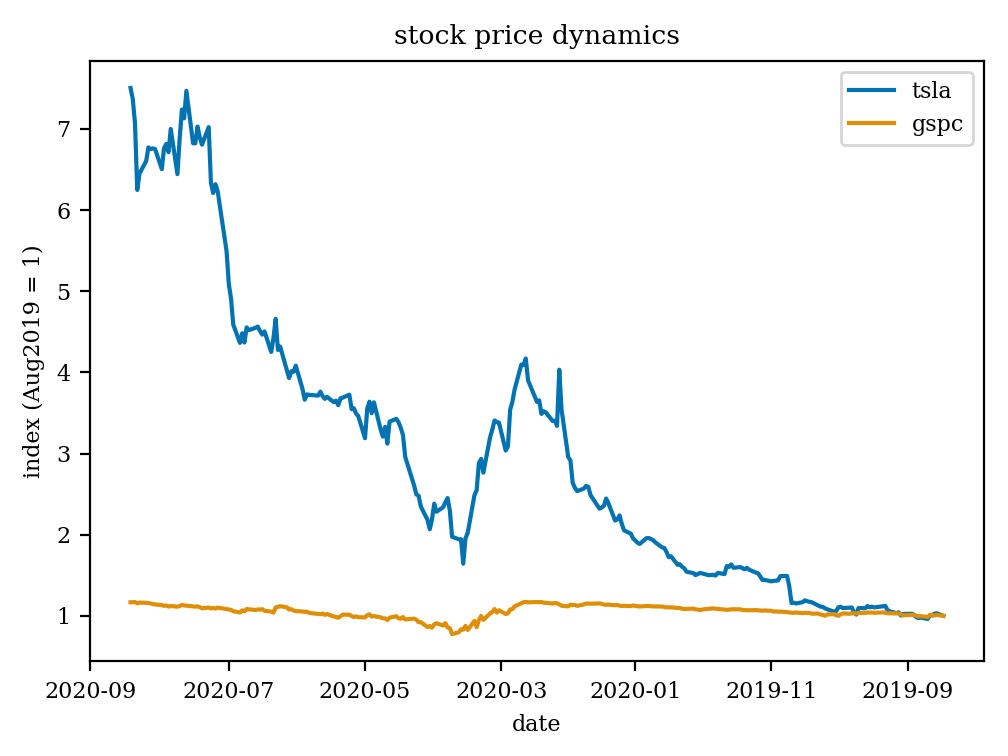
\includegraphics[height=0.5\textheight,width=\linewidth,keepaspectratio]{stock-index-weird-plot}
%                     \caption{First subfigure}
%                 \end{figure}
%             \end{column}
%             \begin{column}{.45\textwidth}
%                 \centering
%                 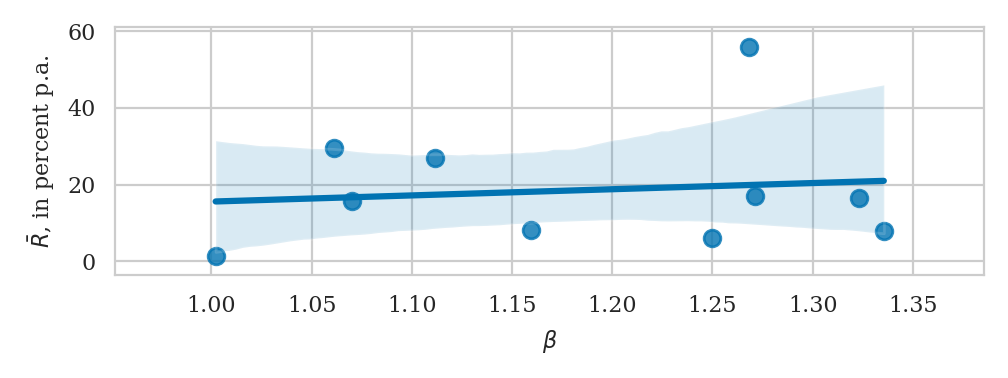
\includegraphics[height=0.5\textheight,width=\linewidth,keepaspectratio]{beta-vs-mu.png}
%                 \caption{Second subfigure}
%             \end{column}    
%         \end{columns}   
%         % \caption{Two panels side by side}
%     \end{figure}
% \end{frame}

\end{document}